\documentclass[xcolor=table]{beamer}
\usepackage[utf8]{inputenc}
\usepackage[british]{babel}
\usepackage[super]{nth}
%\usetheme{Boadilla}
%\usecolortheme{rose}
%\usecolortheme{crane}
%\usefonttheme{structuresmallcapsserif}
%\setbeamertemplate{navigation symbols}{}

\definecolor{Main}{rgb}{0.74, 0.13, 0.19}
\definecolor{Accent1}{rgb}{0.76,0.36,0.13}
\definecolor{Accent2}{rgb}{0.54,0.1,0.4}

\mode<presentation>{\usetheme{ilm}}
%\usecolortheme{rose}
%\useinnertheme[shadow]{circles}
%\usecolortheme{whale}
%\useoutertheme{infolines}

%\usecolortheme[named=Accent1]{structure}




%\setbeamerfont{page number in head/foot}{size=\large}
%\setbeamercolor{page number in head/foot}{fg=Main}
%% page/total
%%\setbeamertemplate{footline}[frame number]
%% pas de total
%\setbeamertemplate{footline}{%
%    	\hfill%
%	\usebeamercolor[fg]{page number in head/foot}%
%	\usebeamerfont{page number in head/foot}%
%	\insertframenumber\kern1em\vskip2pt%
%}
%
%\setbeamersize{text margin left=1em}
%\setbeamersize{text margin right=1em}

\usepackage[overlay,absolute]{textpos}
\setlength{\TPHorizModule}{10mm}
\setlength{\TPVertModule}{\TPHorizModule}
\textblockorigin{10mm}{10mm} % start everything near the top-left corner
\setlength{\parindent}{0pt}

%font
\usepackage[T1]{fontenc}
\usepackage{times}
%\usepackage[oldstylenums]{kpfonts}

%\include{macros}
\usepackage{ifthen}


%proper math and math symbols
\usepackage{amsmath,mathtools}
\usepackage{amssymb}

\usepackage{datenumber,fp}

\usepackage[separate-uncertainty = true]{siunitx}

\usepackage{tabu}
\usepackage{multirow}
\usepackage{booktabs}

% Allow the usage of graphics (.jpg, .png, etc.) in the document
\usepackage{graphicx}
\usepackage{tikz}
\usetikzlibrary{arrows,shapes,backgrounds, calc, positioning, topaths,chains, intersections, decorations.markings, decorations.text, shapes.geometric, matrix,patterns,mindmap,fit}
%\usetikzlibrary{positioning, patterns,topaths,chains,matrix}

\usepackage{pgfplots}
\usepackage{pgfplotstable}
\pgfplotsset{compat=1.9}
\usepgfplotslibrary{fillbetween}
\usepgfplotslibrary{groupplots}
\usepgfplotslibrary{external}
\makeatletter
\newcommand*{\overlaynumber}{\number\beamer@slideinframe}
\tikzset{
  beamer externalizing/.style={%
    execute at end picture={%
      \tikzifexternalizing{%
        \ifbeamer@anotherslide
        \pgfexternalstorecommand{\string\global\string\beamer@anotherslidetrue}%
        \fi
      }{}%
    }%
  },
  external/optimize=false
}
\let\orig@tikzsetnextfilename=\tikzsetnextfilename
\renewcommand\tikzsetnextfilename[1]{\orig@tikzsetnextfilename{#1-\overlaynumber}}
\makeatother

\tikzset{every picture/.style={beamer externalizing}}
\tikzexternalize
\tikzsetexternalprefix{fig_presentation/}
%\tikzset{external/optimize=false}
%\tikzset{external/force remake}


%link or play movies
\usepackage{multimedia}

%chemistry
\usepackage[version=3]{mhchem}
\usepackage{chemfig}
\usepackage{setspace}


%beamer related package

\usepackage{todonotes}
\presetkeys{todonotes}{inline}{}

\tikzset{onslide/.code args={<#1>#2}{%
  \only<#1>{\pgfkeysalso{#2}} %
}}%


%bibliography
\usepackage[style=authoryear-comp, language=british,eprint=false, url=false, doi=false, sortcites=true, sorting=none, isbn=false, firstinits=true,maxcitenames=6]{biblatex}
%minimal citations
\AtEveryCitekey{%
	\clearfield{title}
	\clearfield{pages}
	\clearfield{volume}
	\clearfield{number}
	\clearfield{month}}
\newcommand{\myfullcite}[1]{{\scriptsize\fullcite{#1}}}
\renewbibmacro{in:}{%
  \ifentrytype{article}{}{%
  \printtext{\bibstring{in}\intitlepunct}}}
%\bibliography{biblio}


\newcolumntype{P}[1]{>{\raggedright}p{#1}}

\institute[iLM]{Univ Lyon, Université Claude Bernard Lyon 1, CNRS, Institut Lumière Matière}
\title[processionary gel]{Ion pairing controls rheological properties of ``processionary'' polyelectrolyte hydrogels}
\author[M. Leocmach]{Mathieu Leocmach \hfill{\usebeamerfont{normal text}\texttt{\usebeamercolor[fg]{normal text}\footnotesize @LamSonLeoc\includegraphics[height=1em]{Twitter_Bird}}}\vspace{-\baselineskip}}
\date{%10 August 2016
}
\titlegraphic{\vspace{-\baselineskip}
	\begin{tabu}{X[c]X[c]X[c]X[c]}
		\multicolumn{2}{c}{\usebeamerfont{institute}\usebeamercolor[fg]{institute}ENS de Lyon, Laboratoire de Chimie}&
		\multicolumn{2}{c}{\usebeamerfont{institute}\usebeamercolor[fg]{institute}ENS de Lyon, Laboratoire de Physique}\\\cmidrule(r){1-2}\cmidrule(l){3-4}
		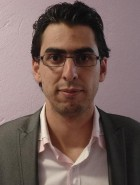
\includegraphics[height=3\baselineskip]{presentation/Hassan}&
		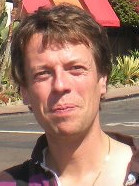
\includegraphics[height=3\baselineskip]{presentation/Cyrille}&
		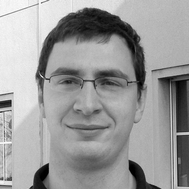
\includegraphics[height=3\baselineskip]{presentation/Nicolas_Taberlet}&
		\includegraphics[height=3\baselineskip]{../Yaourt/Seb}\\
		Hassan & Cyrille & Nicolas & S\'{e}bastien\\
		Srour & Monnereau & Taberlet & Manneville\\\cmidrule(r){1-2}
		\multicolumn{2}{c}{Martien Duvall Deffo Ayagou}&\\
		\multicolumn{2}{c}{Thi Thanh-Tam Nguyen}&\raisebox{-0.1em}[0pt][0pt]{
\includegraphics[height=2\baselineskip]{presentation/invest-avenir.jpg}}&\raisebox{-0.1em}[0pt][0pt]{\includegraphics[height=2\baselineskip,clip=true, trim=6mm 14mm 6mm 0]{../Yaourt/NEW-Logo-ERC-OUTLINE}}\\
	\end{tabu}
	
\bigskip
Martien Duvall Deffo Ayagou, Thi Thanh-Tam Nguyen%, Chantal Andraud
	
	%\vfill
	%\includegraphics[height=2\baselineskip]{logo_ens-lyon}\quad
	%\includegraphics[height=2\baselineskip]{logo_ums_grand}\quad
	%\includegraphics[height=2\baselineskip]{../../Yaourt/CNRSfilaire-Q}\quad
	%\includegraphics[height=2\baselineskip]{CRPP}\quad
	%\includegraphics[height=2\baselineskip,clip=true, trim=6mm 14mm 6mm 0]{NEW-Logo-ERC-OUTLINE}
	}


\newlength{\mylength}

%\includeonly{creep_beamer}

\begin{document}
\tikzset{every mark/.append style={scale=0.8}}
\pgfplotsset{every axis/.append style={footnotesize}}

\pgfplotscreateplotcyclelist{earthy}{%
{red!40!black,mark=o},
{red!60!black,mark=triangle, every mark/.append style={rotate=180}},
{red!80!black,mark=square},
{red,mark=triangle},
{red!80!yellow, mark=diamond},
red!60!yellow,
red!40!yellow,
}

\AtBeginSection[]{
	\addtocounter{framenumber}{-1}
	\begin{frame}[plain]
		\tableofcontents[currentsection, hideothersubsections]
	\end{frame}
}

\begin{frame}{\pgfuseimage{cnrs-logo}\hspace*{0.3cm}\pgfuseimage{ucbl-logo}\pgfuseimage{univlyon-logo}}%[plain]
	\titlepage
\end{frame}

\setcounter{framenumber}{0}

\begin{frame}{What chemists/physicists think I do}
	\begin{columns}[t]
	\column{0.5\textwidth}
	\begin{flushleft}\structure{chemistry}
	
	``This counterion is more chaotropic''
	
	\vspace{\baselineskip}
	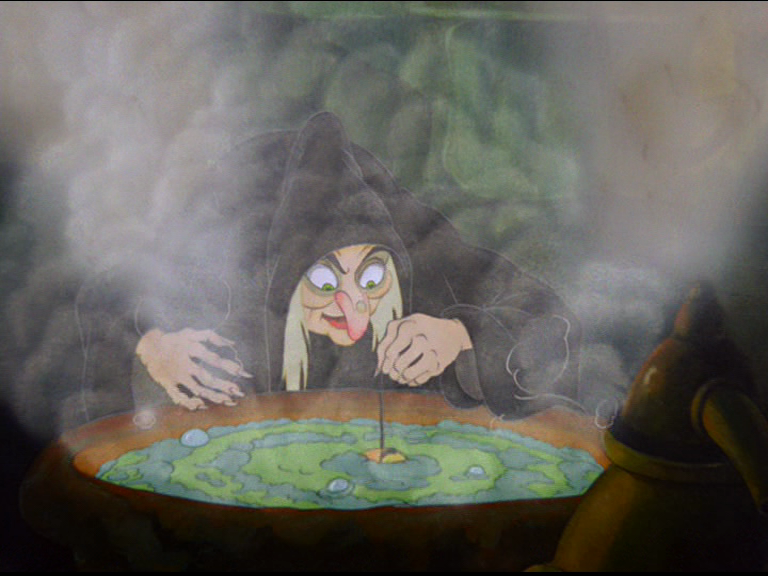
\includegraphics[width=\textwidth]{presentation/sorciere}
	\end{flushleft}
	\column{0.5\textwidth}
	\begin{flushright}\structure{rheology}
	
	``We impose a constant shear stress''
	\end{flushright}
	\hspace{0.25\textwidth}
\includegraphics[height=10\baselineskip]{presentation/rascar}
	\end{columns}
\end{frame}

\begin{frame}{Physical chemistry positive feedback}
\tikzsetnextfilename{chem_rheol}%
	\definesubmol{head}{(-[::-105,,,,ilmcolor])(-[::-15,,,,ilmcolor])-[::60,,,,ilmcolor](=[::60,,,,ilmcolor]\textcolor{ilmcolor}{O})-[::-60,,,,ilmcolor]\textcolor{ilmcolor}{O}-[::-60,,,,ilmcolor]-[::60,,,,ilmcolor]-[::60,,,,ilmcolor]}
\definesubmol{mono}{-[::-60,,,,gray](=[,,,,gray]\textcolor{gray}{O}(-[,1.5,,,densely dotted]\textcolor{cyan!60!black}{H}-[,1.25,,,cyan!60!black]\textcolor{cyan!60!black}{O}(-[1,1,,,draw=none]\textcolor{red}{\delta^{-}})-[::-40,1.25,,,cyan!60!black]\textcolor{cyan!60!black}{H}?-[0,1,,,draw=none]\textcolor{red}{\delta^{+}}))-[::-60,,,,gray]\textcolor{gray}{O}-[::60,,,,gray]-[,,,,gray]-[::-60,,,,gray]}
\begin{tikzpicture}
%axis and rheometer
\draw[-stealth] (0,0) -- (\textwidth,0) node[below left]{\si{\metre}} node[above left=1em and 0] (rheo) {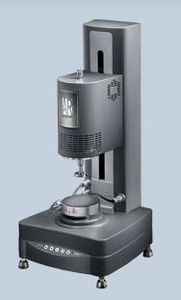
\includegraphics[width=0.15\textwidth]{presentation/rheo_ar1000.jpg}} \foreach \x in {-10,-9,...,-2}{node[pos=(\x+11)/10, label={[font=\footnotesize]-90:10\textsuperscript{\x}}] {|}};
\begin{scope}[every node/.style={font=\tiny\setatomsep{1.5em}}]
\node[above right=2em and 0] (PNuX) {%
\chemfig{[:-30]-[@{left,0.25}](%
	!{mono}\textcolor{ilmorange}{Nu^{+}}-[0,2,,,draw=none]\textcolor{blue!80!black}{X^{-}}?[,,densely dotted]%
	)-[::60]-[@{right,0.25}]!{head}\textcolor{ilmcolor}{P}|\textcolor{ilmcolor}{O_3^{2-}}}%
};
  \node[below right=-0.6em and -0.25em of PNuX.base west] {$\prescript{}{N_0}{\left[\vrule height 1em depth 0.25em width 0pt\hspace{1.75em}\right]}$};
\end{scope}
\draw[thick,-stealth] (rheo) to[bend right] (PNuX) node[ilmorange] at (0.5\textwidth,8em){understand};
\draw[thick,-stealth] (PNuX) to[bend right] (rheo) node[ilmorange] at (0.5\textwidth,2em){design};
\node[above=0 of rheo,ilmcolor] (rhl){rheology};
\node[anchor=base,ilmcolor] at (PNuX.north|-rhl.base) {chemistry};
\end{tikzpicture}
\end{frame}

\begin{frame}{Fine chemistry}
	\vspace{\baselineskip}
	\tikzsetnextfilename{polymerisation}%
	\let\mrad\relax%
	\newlength\mrad%
	\setlength{\mrad}{1ex}%
	% The face style, can be changed
	\tikzset{face/.style={
		shape=circle,minimum size=2\mrad,shading=radial,outer sep=0pt,
	    inner color=white!50!yellow,outer color= yellow!70!orange
		}}%
	\begin{tikzpicture}
		\foreach \i [evaluate=\i as \dist using \i*0.45] in {0,1,2}{
			\begin{scope}[xshift=\dist\textwidth]
			%face
			\begin{scope}[face/.style={
		shape=circle,minimum size=2\mrad,shading=radial,outer sep=0pt,
	    inner color=white!50!yellow,outer color= yellow!70!orange
		}]
\node[face,inner color=white!50!ilmcolor,outer color= ilmcolor!90!black] (emoticon) {};
			%% The eyes are fixed.
			\draw[fill=white] 
				(-0.5\mrad,0ex) ..controls (-0.25\mrad,0.1\mrad)and(0.25\mrad,0.1\mrad)..
		        (0.5\mrad,0.0pt) ..controls (0.75\mrad,0.75\mrad)and(0.1\mrad,0.85\mrad)..
		        (0pt,0.2\mrad) ..controls (-0.1\mrad,0.85\mrad)and(-0.75\mrad,0.75\mrad)..
		        (-0.5\mrad,0pt)--cycle;
			%% standard pupils
			\node[fill, ellipse,inner xsep=0.075\mrad, inner ysep=0.0375\mrad, rotate=80] at (0.25\mrad,0.25\mrad) {};
			\node[fill, ellipse,inner xsep=0.075\mrad, inner ysep=0.0375\mrad, rotate=100] at (-0.25\mrad,0.25\mrad) {};
			%% mouth
			\draw[thick,line cap=round] (-0.5\mrad,-0.5\mrad)
			     ..controls (-0.25\mrad,-0.75\mrad)and(0.25\mrad,-0.75\mrad)..(0.5\mrad,-0.5\mrad);
\end{scope}
;
			%% horns
			\draw[every node/.style={shape=circle,inner sep=0.2\mrad,shading=radial,inner color=white!50!ilmcolor,outer color= ilmcolor!90!black}] (emoticon.70) -- ++(70:0.4\mrad) node{} (emoticon.110) -- ++(110:0.4\mrad) node{};
			%\draw ( emoticon.80)..controls ( 0.3\mrad,1.2\mrad)..(0.5\mrad,1.25\mrad)
			      %..controls ( 0.4\mrad,1.15\mrad)..(emoticon.70);
			%\draw (emoticon.100)..controls (-0.3\mrad,1.2\mrad)..(-0.5\mrad,1.25\mrad)
			      %..controls (-0.4\mrad,1.15\mrad)..(emoticon.110);
			%body segments
			\ifthenelse{\i=0}{}{
			\foreach \x in {0,2,...,10}{
				\node[face,inner color=white!50!gray,outer color= gray!90!black, left=\x\mrad of emoticon] (monomer){};
				%legs
				\ifthenelse{\i=1}{}{
					\draw[line width=0.25\mrad, ilmorange] (monomer.south) ++(0,0.5\mrad) to[bend left] +(0,-1\mrad);}
			};}
			\ifthenelse{\i=1}{
				\draw[|-|] ($(monomer.west)+(0,-1.5\mrad)$) -- ($(emoticon.west)+(0,-1.5\mrad)$) node[midway,below, font=\scriptsize] {$N_0$};
			}{}
			\end{scope}
			};
			%arrows
			\draw[-stealth, thick] ++(3\mrad,0) -- +(6\mrad,0) node[midway, above=0.2\mrad, face,inner color=white!50!gray,outer color= gray!90!black]{} node[midway, below, font=\scriptsize]{ATRP};
			\draw[-stealth, thick] ++(0.45\textwidth,0) ++(3\mrad,0) -- +(6\mrad,0) coordinate[midway, above=0.2\mrad] (leg) node[midway, below, font=\scriptsize,text width=10\mrad,align=center]{post-functionalization};
			\draw[line width=0.25\mrad, ilmorange] (leg) to[bend right] +(0,1\mrad);
		\end{tikzpicture}

	\bigskip
	\tikzsetnextfilename{polymerisation_PImBr}%
	\definesubmol{head}{(-[::-105,,,,ilmcolor])(-[::-15,,,,ilmcolor])-[::60,,,,ilmcolor](=[::60,,,,ilmcolor]\textcolor{ilmcolor}{O})-[::-60,,,,ilmcolor]\textcolor{ilmcolor}{O}-[::-60,,,,ilmcolor]-[::60,,,,ilmcolor]-[::60,,,,ilmcolor]}
\definesubmol{mono}{-[::-60,,,,gray](=[,,,,gray]\textcolor{gray}{O})-[::-60,,,,gray]\textcolor{gray}{O}-[::60,,,,gray]-[,,,,gray]-[::-60,,,,gray]}
\tikzsetnextfilename{polymerisation_PImBr}
\begin{tikzpicture}[every node/.style={font=\tiny\setatomsep{1.5em}}]
	\node (init) {\chemfig{Br-[:-30]!{head}\textcolor{ilmcolor}{P}|\textcolor{ilmcolor}{O_3}Et_2}};
	
	\node[below left=5\baselineskip and 0 of init.east] (POH) {%
	\chemfig{[:-30]-[@{left,0.25}](%
		!{mono}OH%
		)-[::60,,,,gray]-[@{right,0.25}]!{head}\textcolor{ilmcolor}{P}|\textcolor{ilmcolor}{O_3}Et_2}%
	};
	\node[below right=-0.6em and -0.25em of POH.base west] {$\prescript{}{N_0}{\left[\vrule height 1em depth 0.25em width 0pt\hspace{1.75em}\right]}$};
	\node[below right=-0.6em and -0.25em of POH.base west] {};
	
	\node[right=0.1\textwidth of init.base east, anchor=base west] (PBr) {%
	\chemfig{[:-30]-[@{left,0.25}](%
		!{mono}Br%
		)-[::60,,,,gray]-[@{right,0.25}]!{head}\textcolor{ilmcolor}{P}|\textcolor{ilmcolor}{O_3^{2-}}}%
	};
	\node[below right=-0.6em and -0.25em of PBr.base west] {$\prescript{}{N_0}{\left[\vrule height 1em depth 0.25em width 0pt\hspace{1.75em}\right]}$};
	
	\node[right=\textwidth of init.base-|POH.west, anchor=base east] (PNuBr) {%
	\chemfig{[:-30]-[@{left,0.25}](%
		!{mono}\textcolor{ilmorange}{N}|^{\color{ilmorange}+}*5(=[,,,,thick, ilmorange]-[,,,,thick, ilmorange]\textcolor{ilmorange}{N}(-[,,,,thick, ilmorange])-[,,,,thick, ilmorange]=[,,,,thick, ilmorange]-[,,,,thick, ilmorange])(-[0,2,,,draw=none]Br^{-})
		)-[::60,,,,gray]-[@{right,0.25}]!{head}\textcolor{ilmcolor}{P}|\textcolor{ilmcolor}{O_3^{2-}}}%
	};
	\node[below right=-0.6em and -0.25em of PNuBr.base west] {$\prescript{}{N_0}{\left[\vrule height 1em depth 0.25em width 0pt\hspace{1.75em}\right]}$};
	
	\draw[-stealth, thick] (init.south-|POH.north) -- (POH) node[midway, left=0, -]{\chemfig{[:-30]=[,,,,gray]!{mono}OH}} node[midway, right=0, text width=0.13\textwidth, align=center]{\ce{CuBr}\linebreak 4-4'-bipyridine\linebreak \SI{85}{\celsius}};
	\draw[-stealth, thick] (POH) -| (PBr) node[pos=0.25, above]{\ce{TMS-Br}} node[pos=0.25, below, sloped, text width=0.2\textwidth, align=center]{\ce{CH2Cl2}\linebreak \SI{85}{\celsius}};
	\draw[-stealth, thick] (PBr) -- (PBr-|PNuBr.west) node[midway, above,align=center,-]{\chemfig[thick, ilmorange]{[2]*5(-N(-)-=N-=)}} node[midway, below, text width=0.2\textwidth, align=center]{THF\linebreak \SI{85}{\celsius}};;
	\node[anchor=south east] at (POH.south east) {\ce{POH}};
	\node[anchor=south east] at (PBr.south east) {\ce{PBr}};
	\node[anchor=south east] at (PNuBr.south east) {\ce{PIm+Br-}};
	\node[anchor=south east, font=\footnotesize] at (POH.south-|PNuBr.east) {$N_0=70$ from NMR};
\end{tikzpicture}
\end{frame}

\begin{frame}{Physical polyelectrolytes hydrogel}
	\tikzsetnextfilename{polyelectrolytes}%
\begin{tikzpicture}
\let\mrad\relax%
\newlength\mrad%
\setlength{\mrad}{0.45em}%
\draw[every node/.style={circle,draw,font=\tiny, inner sep=0,minimum height=0.5em}] (0,0) --(30:\mrad) node[above right,ilmcolor]{-} (0,0)--(-30:\mrad) node[below right,ilmcolor]{-} (0,0)--++(-180:\mrad)\foreach \x [evaluate=\x as \r using 1/(rnd+0.1), evaluate=\x as \rr using 1/(rnd+0.1)] in {1,2,...,35}{--++(150:\mrad)node[above,ilmorange]{+} node[above=\r\mrad]{-}--++(-150:\mrad)node[below=0,ilmorange]{+} node[below=\rr\mrad]{-}};
\end{tikzpicture}%
\begin{columns}
\column{0.5\textwidth}
\structure{Reversible gel}
\begin{itemize}
	\item in deionised, neutral water
	\item yield stress fluid
\end{itemize}
\structure{Solution} if
\begin{itemize}
	\item ionic strength, pH
	\item non ionic head
\end{itemize}
$\Rightarrow$ Head-to-body ionic bonds

\column{0.5\textwidth}
\hfill Herschel-Bulkley law\\
\hfill $\sigma =\sigma_c + A \dot{\gamma}^n$
\tikzsetnextfilename{flowcurves}%
\begin{tikzpicture}
    \let\mrad\relax%
	\newlength\mrad%
	\setlength{\mrad}{0.5em}%
% The face style, can be changed
	\tikzset{face/.style={
		shape=circle,minimum size=2\mrad,shading=radial,outer sep=0pt,
	    inner color=white!50!yellow,outer color= yellow!70!orange
		}}%
\let\drawcaterpillar\relax
\newcommand\drawcaterpillar{
			%face
			\node[face,inner color=white!50!ilmcolor,outer color= ilmcolor!90!black] (emoticon) {};
			%% The eyes are fixed.
			\draw[fill=white] 
				(-0.5\mrad,0ex) ..controls (-0.25\mrad,0.1\mrad)and(0.25\mrad,0.1\mrad)..
		        (0.5\mrad,0.0pt) ..controls (0.75\mrad,0.75\mrad)and(0.1\mrad,0.85\mrad)..
		        (0pt,0.2\mrad) ..controls (-0.1\mrad,0.85\mrad)and(-0.75\mrad,0.75\mrad)..
		        (-0.5\mrad,0pt)--cycle;
			%% standard pupils
			\node[fill, ellipse,inner xsep=0.075\mrad, inner ysep=0.0375\mrad, rotate=80] at (0.25\mrad,0.25\mrad) {};
			\node[fill, ellipse,inner xsep=0.075\mrad, inner ysep=0.0375\mrad, rotate=100] at (-0.25\mrad,0.25\mrad) {};
			%% mouth
			\draw[thick,line cap=round] (-0.5\mrad,-0.5\mrad)
			     ..controls (-0.25\mrad,-0.75\mrad)and(0.25\mrad,-0.75\mrad)..(0.5\mrad,-0.5\mrad);
			
%body segments
			\foreach \x in {0,2,...,4}{
				\node[face,inner color=white!50!gray,outer color= gray!90!black, left=\x\mrad of emoticon] (monomer){};
				%legs
				\draw[line width=0.25\mrad, ilmorange] (monomer.south) ++(0,0.5\mrad) to[bend left] +(0,-1\mrad);
			};
}
\begin{loglogaxis}[
	name=ax,
	xlabel=$\dot\gamma\,(\si{\per\second})$,
	ylabel={$\sigma$ (\si{\pascal)}},
	clip marker paths=true,
	]
	\addplot+[mark=o] table[x=shear_rate, y=shear_stress] {data/PO3-P60-Im+-0pc-02-06-14_8pcw_flow curve_down.txt};
	\addplot+[mark=square] table[x=shear_rate, y=shear_stress] {data/PO3-P60-Im+-0pc-02-06-14_22pcw_flow curve_down.txt};
	\addplot+[black] table[x=shear_rate, y=shear_stress,skip coords between index={0}{20}] {data/Et-P60-Im+-0pc-21-05-14_10pcw_flow_curve_down.txt};
	\addplot[domain=2e-2:5e2]{0.47+1.19*x^0.7};
	\addplot[domain=2e-2:5e2]{7.5+15.1*x^0.62};
\end{loglogaxis}

\begin{scope}[shift=(ax.north), yshift=-2\mrad, xshift=-\mrad]
			\drawcaterpillar
			%% horns
			\draw[every node/.style={shape=circle,inner sep=0.2\mrad,shading=radial,inner color=white!50!ilmcolor,outer color= ilmcolor!90!black}] (emoticon.70) -- ++(70:0.4\mrad) node{} (emoticon.110) -- ++(110:0.4\mrad) node{};
\end{scope}
\begin{scope}[shift=(ax.south), yshift=2\mrad, xshift=-\mrad]
			\drawcaterpillar
\end{scope}
\end{tikzpicture}
\end{columns}
\vspace{-\baselineskip}\textit{\scriptsize Srour et al. Macromol. Rapid Comm., 36, 55 (2015)}
\end{frame}

\begin{frame}{Linear rheology}
	\begin{columns}
	\column{0.5\textwidth}
	\tikzsetnextfilename{linear_rheology_PImBr}%
	\begin{tikzpicture}
	\pgfplotscreateplotcyclelist{moduli}{
		black, mark=*\\%
		black, mark=square\\%
	}
	\begin{loglogaxis}[
		ylabel={moduli (\si{\pascal})},
		xlabel={frequency (\si{\hertz})},
		cycle list name=moduli,
		ytickten={0, 1}, yticklabels={1,10},
		]
		\addplot table[x expr={\thisrow{angfrequency}/6.28}, y=G']{ImBr_70_PO3_8pc_ter.freq} node[midway, above left]{$G^\prime$};
		\addplot table[x expr={\thisrow{angfrequency}/6.28}, y=G'']{ImBr_70_PO3_8pc_ter.freq}  node[midway, below right]{$G^{\prime\prime}$};
		\node[anchor=north west, font=\footnotesize] at (rel axis cs:0,1){8\% wt};
	\end{loglogaxis}
\end{tikzpicture}
	\[ G = \frac{c}{N}k_\mathrm{B}T \]
	\begin{description}[$N$]
	\item[$c$] monomer concentration
	\item[$N$] \# monomers between CL
	\end{description}
	\column{0.45\textwidth}
	\pause
	\begin{itemize}
	\item $N \approx 800 N_0$ !
	\item 800 chains between CL
	\end{itemize}
	\begin{flushright}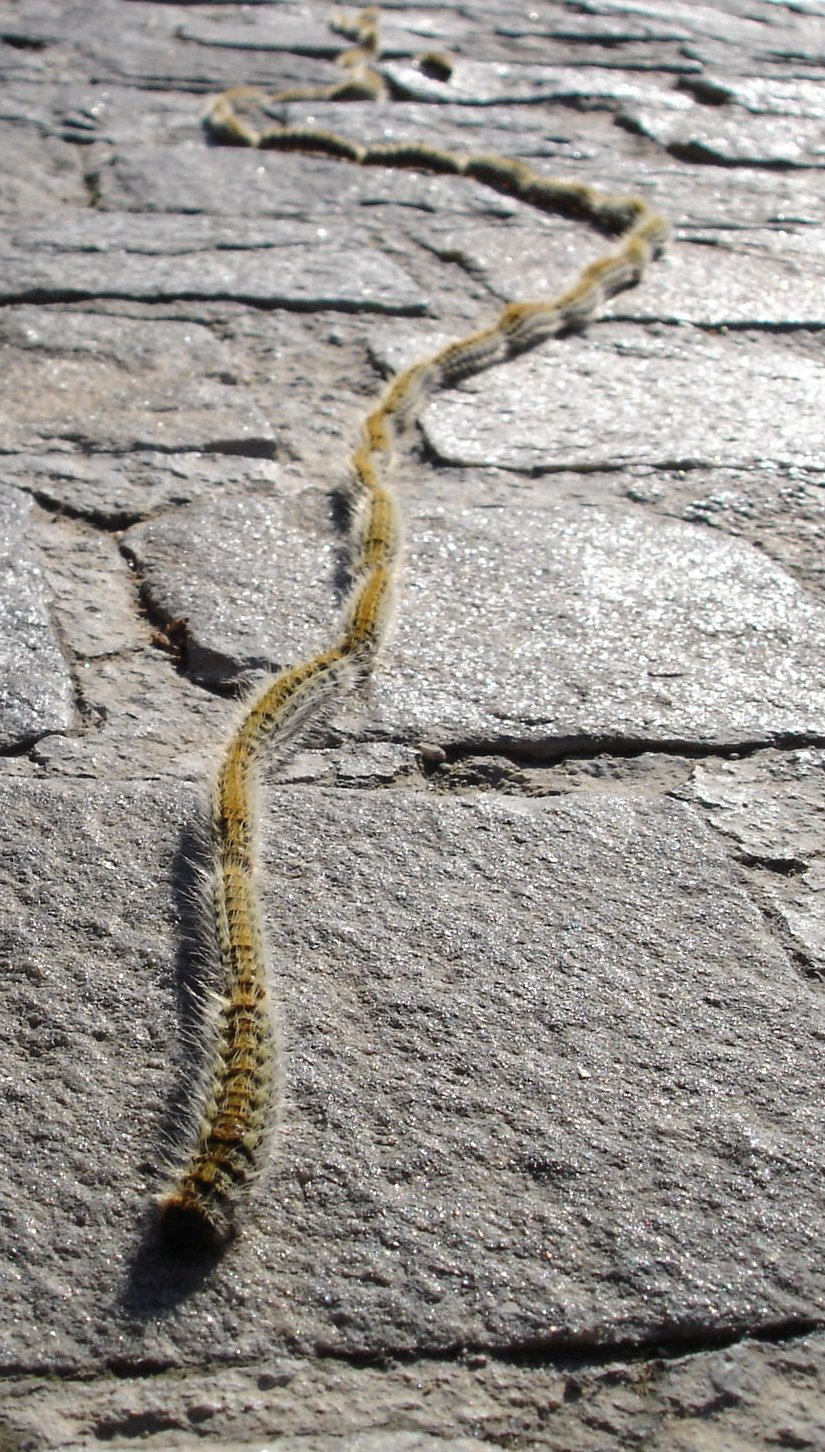
\includegraphics[height=14\baselineskip]{presentation/Thaumetopea_pityocampa_01.jpg}\\
	\vspace{-1.5em}\colorbox{lightgray}{\scriptsize Wikimedia commons}
	\end{flushright}
	\end{columns}
\end{frame}

\begin{frame}{Tweaking repeated ions + counterions}
	\vspace{1.5\baselineskip}
	\tikzsetnextfilename{postfunc}%
	\let\mrad\relax%
	\newlength\mrad%
	\setlength{\mrad}{1ex}%
	% The face style, can be changed
	\tikzset{face/.style={
		shape=circle,minimum size=2\mrad,shading=radial,outer sep=0pt,
	    inner color=white!50!yellow,outer color= yellow!70!orange
		}}%
	\begin{tikzpicture}
		\foreach \i [evaluate=\i as \dist using (floor(\i/2))*0.425, evaluate=\i as \ys using 1.5*(\i-2*floor(\i/2))] in {1,2,3,4,5}{
			\begin{scope}[xshift=\dist\textwidth, yshift=\ys\baselineskip]
			
			%face
			\node[inner sep=0] (emoticon) {\begin{scope}[face/.style={
		shape=circle,minimum size=2\mrad,shading=radial,outer sep=0pt,
	    inner color=white!50!yellow,outer color= yellow!70!orange
		}]
\node[face,inner color=white!50!ilmcolor,outer color= ilmcolor!90!black] (emoticon) {};
			%% The eyes are fixed.
			\draw[fill=white] 
				(-0.5\mrad,0ex) ..controls (-0.25\mrad,0.1\mrad)and(0.25\mrad,0.1\mrad)..
		        (0.5\mrad,0.0pt) ..controls (0.75\mrad,0.75\mrad)and(0.1\mrad,0.85\mrad)..
		        (0pt,0.2\mrad) ..controls (-0.1\mrad,0.85\mrad)and(-0.75\mrad,0.75\mrad)..
		        (-0.5\mrad,0pt)--cycle;
			%% standard pupils
			\node[fill, ellipse,inner xsep=0.075\mrad, inner ysep=0.0375\mrad, rotate=80] at (0.25\mrad,0.25\mrad) {};
			\node[fill, ellipse,inner xsep=0.075\mrad, inner ysep=0.0375\mrad, rotate=100] at (-0.25\mrad,0.25\mrad) {};
			%% mouth
			\draw[thick,line cap=round] (-0.5\mrad,-0.5\mrad)
			     ..controls (-0.25\mrad,-0.75\mrad)and(0.25\mrad,-0.75\mrad)..(0.5\mrad,-0.5\mrad);
\end{scope}
};
			%% horns
			\draw[every node/.style={shape=circle,inner sep=0.2\mrad,shading=radial,inner color=white!50!ilmcolor,outer color= ilmcolor!90!black}] (emoticon.70) -- ++(70:0.4\mrad) node{} (emoticon.110) -- ++(110:0.4\mrad) node{};
			%\draw ( emoticon.80)..controls ( 0.3\mrad,1.2\mrad)..(0.5\mrad,1.25\mrad)
			      %..controls ( 0.4\mrad,1.15\mrad)..(emoticon.70);
			%\draw (emoticon.100)..controls (-0.3\mrad,1.2\mrad)..(-0.5\mrad,1.25\mrad)
			      %..controls (-0.4\mrad,1.15\mrad)..(emoticon.110);
			%body segments
			
			\foreach \x in {0,2,...,8}{
				\node[face,inner color=white!50!gray,outer color= gray!90!black, left=\x\mrad of emoticon] (monomer){};
				%legs
				\ifthenelse{\i=3}{
					\draw[line width=0.25\mrad, ilmorange] (monomer.south) ++(0,0.5\mrad) to[bend left] +(0,-1\mrad);}{}
				\ifthenelse{\i=2}{
					\node[circle, inner sep=0.3\mrad, fill=ilmorange] at (monomer.south){};}{}
				\ifthenelse{\i=5}{
					\draw[line width=0.25\mrad, blue!80!black] (monomer.south) ++(0,0.5\mrad) to[bend left] +(0,-1\mrad);}{}
				\ifthenelse{\i=4}{
					\node[circle, inner sep=0.3\mrad, fill=blue!80!black] at (monomer.south){};}{}
			};
			\end{scope}
			};
			%arrows
			%\draw[-stealth, thick] ++(3\mrad,0) -- +(6\mrad,0) node[midway, above=0.2\mrad, face,inner color=white!50!gray,outer color= gray!90!black]{} node[midway, below, font=\scriptsize]{ATRP};
			\draw[-stealth, thick] ++(3\mrad,1.5\baselineskip) -- +(6\mrad,0) coordinate[midway, above=0.2\mrad] (leg) node[midway, below, font=\scriptsize,text width=10\mrad,align=center]{post-functionalization};
			\draw[line width=0.25\mrad, ilmorange] (leg) to[bend right] +(0,1\mrad);
			\draw[-stealth, thick] ++(3\mrad,0) -- +(6\mrad,0) node[midway, below=0.2\mrad, circle, inner sep=0.3\mrad, fill=ilmorange] (leg){};
			\draw[-stealth, thick] ++(0.425\textwidth,0) ++(3\mrad,0.75\baselineskip) -- +(6\mrad,0) coordinate[midway, above=0.2\mrad] (leg) node[midway, above, font=\scriptsize]{counterion} node[midway, below, font=\scriptsize,text width=10\mrad,align=center]{exchange};
		\end{tikzpicture}

	\bigskip
	\tikzsetnextfilename{postfunc_chem}%
	\definesubmol{head}{(-[::-105,,,,ilmcolor])(-[::-15,,,,ilmcolor])-[::60,,,,ilmcolor](=[::60,,,,ilmcolor]\textcolor{ilmcolor}{O})-[::-60,,,,ilmcolor]\textcolor{ilmcolor}{O}-[::-60,,,,ilmcolor]-[::60,,,,ilmcolor]-[::60,,,,ilmcolor]}
\definesubmol{mono}{-[::-60,,,,gray](=[,,,,gray]\textcolor{gray}{O})-[::-60,,,,gray]\textcolor{gray}{O}-[::60,,,,gray]-[,,,,gray]-[::-60,,,,gray]}
\begin{tikzpicture}[every node/.style={font=\tiny\setatomsep{1.5em}}]
	
	\node (PBr) {%
	\chemfig{[:-30]-[@{left,0.25}](%
		!{mono}Br%
		)-[::60,,,,gray]-[@{right,0.25}]!{head}\textcolor{ilmcolor}{P}|\textcolor{ilmcolor}{O_3^{2-}}}%
	};
	\node[below right=-0.6em and -0.25em of PBr.base west] {$\prescript{}{N_0}{\left[\vrule height 1em depth 0.25em width 0pt\hspace{1.75em}\right]}$};
	
	\node[right=0.05\textwidth of PBr, yshift=3\baselineskip] (PImBr) {%
	\chemfig{[:-30]-[@{left,0.25}](%
		!{mono}\textcolor{ilmorange}{N}|^{\color{ilmorange}+}*5(=[,,,,thick, ilmorange]-[,,,,thick, ilmorange]\textcolor{ilmorange}{N}(-[,,,,thick, ilmorange])-[,,,,thick, ilmorange]=[,,,,thick, ilmorange]-[,,,,thick, ilmorange])(-[0,2,,,draw=none]Br^{-})
		)-[::60,,,,gray]-[@{right,0.25}]!{head}\textcolor{ilmcolor}{P}|\textcolor{ilmcolor}{O_3^{2-}}}%
	};
	\node[below right=-0.6em and -0.25em of PImBr.base west] {$\prescript{}{N_0}{\left[\vrule height 1em depth 0.25em width 0pt\hspace{1.75em}\right]}$};

	\node[right=0.05\textwidth of PBr, yshift=-3\baselineskip] (PPyrBr) {%
	\chemfig{[:-30]-[@{left,0.25}](%
		!{mono}\textcolor{ilmorange}{N}|^{\color{ilmorange}+}*5([5](-[,,,,thick, ilmorange])-[,,,,thick, ilmorange]-[,,,,thick, ilmorange]-[,,,,thick, ilmorange]-[,,,,thick, ilmorange]-[,,,,thick, ilmorange])(-[:-30,2,,,draw=none]Br^{-})
		)-[::60,,,,gray]-[@{right,0.25}]!{head}\textcolor{ilmcolor}{P}|\textcolor{ilmcolor}{O_3^{2-}}}%
	};
	\node[below right=-0.6em and -0.25em of PPyrBr.base west] {$\prescript{}{N_0}{\left[\vrule height 1em depth 0.25em width 0pt\hspace{1.75em}\right]}$};

	\node[right=\columnwidth of PBr.base west, anchor=base east] (PNuX) {%
\chemfig{[:-30]-[@{left,0.25}](%
	!{mono}\textcolor{ilmorange}{Nu^{+}}-[0,2,,,draw=none]\textcolor{blue!80!black}{X^{-}}%
	)-[::60]-[@{right,0.25}]!{head}\textcolor{ilmcolor}{P}|\textcolor{ilmcolor}{O_3^{2-}}}%
};

	\draw[decoration=brace, decorate] (PImBr.north east) -- (PPyrBr.south east-|PImBr.east) node[midway] (PNuBr){};
	
	
	\draw[-stealth, thick] (PBr) |- (PImBr.west) node[pos=0.75, above,align=center,-]{\chemfig[thick, ilmorange]{[2]*5(-N(-)-=N-=)}} node[pos=0.75, below, text width=0.2\textwidth, align=center]{THF\linebreak \SI{85}{\celsius}};
	\draw[-stealth, thick] (PBr) |- (PPyrBr.west) node[pos=0.75, above,align=center,-]{\chemfig[thick, ilmorange]{[2]*5(--N(-)---)}} node[pos=0.75, below, text width=0.2\textwidth, align=center]{THF\linebreak \SI{85}{\celsius}};
	\draw[-stealth, thick] (PNuBr) -- (PNuX.west|-PNuBr) node[midway, above, -]{Na\textcolor{blue!80!black}{X}} node[midway, below, text width=0.2\textwidth, align=center]{\ce{H2O}};
	\node[anchor=north] at (PBr.center) {\ce{PBr}};
	\node[anchor=south east] at (PImBr.south east) {\ce{PIm+Br-}};
	\node[anchor=south east] at (PPyrBr.south east) {\ce{PPyr+Br-}};
	\node[anchor=south east] at (PNuX.south east) {\ce{PNu+X-}};
	\node[anchor=north east, blue!80!black] at (PNuX.north west) {X: F, Cl or I};
\end{tikzpicture}
\end{frame}

\begin{frame}<1>[label=condensationranking]{Counterion condensation}
	\tikzsetnextfilename{solubility}%
	\begin{tikzpicture}
\pgfdeclarelayer{background}
\pgfdeclarelayer{foreground}
\pgfsetlayers{background,main,foreground}
\node {PBr} [->, level distance=8em, font=\footnotesize] 
	child [grow=-15] {node(PImBr) {\ce{PIm+Br-}} [level distance=5em]
		child[grow=-30] {node(PImF) {\ce{PIm+F-}}} 
		child[grow=east] {node(PImCl) {\ce{PIm+Cl-}}} 
		child[grow=west] {node(PImI) {\ce{PIm+I-}}}} 
	child [grow=-165] {node(PPyrBr) {\ce{PPyr+Br-}} [level distance=5em]
		child[grow=-30] {node(PPyrF) {\ce{PPyr+F-}}} 
		child[grow=east] {node(PPyrCl) {\ce{PPyr+Cl-}}} 
		child[grow=west] {node(PPyrI) {\ce{PPyr+I-}}}};
\begin{pgfonlayer}{background}
	\draw<2>[ilmorange, line width=0.3em, -stealth,rounded corners] (PImI.base) -- (PImBr.base) -- (PImCl.base) -- (PImF);
	\draw<2>[ilmorange, line width=0.3em, -stealth,rounded corners] (PPyrI.base) -- (PPyrBr.base) -- (PPyrCl.base) -- (PPyrF);
	\draw<3>[ilmorange, line width=0.3em, -stealth,rounded corners] (PPyrI.base) -- (PPyrBr.base) -- (PPyrCl.base) -- (PImI.base) -- (PImBr.base);
\end{pgfonlayer}
	\foreach \x in {PImF,PImCl,PPyrF}{
	\draw<1->[ilmcolor] (\x.north west) -- (\x.base east) (\x.north east) -- (\x.base west) ;
	}
\end{tikzpicture}
	\begin{itemize}
		\item Too much condensation prevents dissolution
		\begin{itemize}
			\item water poor solvent for polymer backbone
			\item polyelectrolytes solubilized by electrostatic repulsion
		\end{itemize}
		\item<2-> Direct Hoffmeister series $\ce{I-}\alert{<}\ce{Br-}\alert{<}\ce{Cl-}\alert{<}\ce{F-}$\\
	\hfill\textit{\scriptsize Hofmeister 1888; Zhang Annu Rev Phys Chem 2010; Schwierz Langmuir 2010}
		\item<3-> \ce{\pi+-\pi+} interactions trap counterions\raisebox{-0.5em}{%
			\begin{tikzpicture}[every node/.style={inner ysep=0,font=\tiny\setatomsep{1.5em}}]
			\node[left=0.5em] (Pyr){\chemfig{[0]*5(--N(-)---)}};
			\node[right=0.5em] (Im){\chemfig{[2]*5(-N(-)-=N-=)}};
			\node[font=\normalsize]{$\alert{<}$};
			\end{tikzpicture}}\\
			\hfill\textit{\scriptsize
			Geronimo PCCP 2011;
			Matthews PCCP 2014;
			Gao J Mol Graph Model 2015}
	\end{itemize}
\end{frame}

\begin{frame}{Condensation and solubility}
	\begin{itemize}
		\item All counterions condensed $\Rightarrow$ neutral $\Rightarrow$ not soluble
	\end{itemize}
	\tikzsetnextfilename{polyelectrolytes_condensed}%
	\begin{tikzpicture}
\let\mrad\relax%
\newlength\mrad%
\setlength{\mrad}{0.45em}%
\draw[every node/.style={circle,draw,font=\tiny, inner sep=0,minimum height=0.5em}] (0,0) --(30:\mrad) node[above right,ilmcolor](antenne){-} (0,0)--(-30:\mrad) node[below right,ilmcolor]{-} (0,0)--++(-180:\mrad)\foreach \x in {1,2,...,35}{--++(150:\mrad)node[above,ilmorange]{+} node[above=0.5em]{-}--++(-150:\mrad)node[below=0,ilmorange]{+} node[below=0.5em]{-}};
\end{tikzpicture}%
	\begin{itemize}
		\item ``Enough'' free counterions $\Rightarrow$ repulsion $\Rightarrow$ soluble
	\end{itemize}
	\tikzsetnextfilename{polyelectrolytes}%
	\begin{tikzpicture}
\let\mrad\relax%
\newlength\mrad%
\setlength{\mrad}{0.45em}%
\draw[every node/.style={circle,draw,font=\tiny, inner sep=0,minimum height=0.5em}] (0,0) --(30:\mrad) node[above right,ilmcolor]{-} (0,0)--(-30:\mrad) node[below right,ilmcolor]{-} (0,0)--++(-180:\mrad)\foreach \x [evaluate=\x as \r using 1/(rnd+0.1), evaluate=\x as \rr using 1/(rnd+0.1)] in {1,2,...,35}{--++(150:\mrad)node[above,ilmorange]{+} node[above=\r\mrad]{-}--++(-150:\mrad)node[below=0,ilmorange]{+} node[below=\rr\mrad]{-}};
\end{tikzpicture}%
\end{frame}

\againframe<2-3>{condensationranking}


\begin{frame}{\# chains between cross links}%
	\tikzsetnextfilename{frequency}%
	\begin{tikzpicture}
\pgfplotscreateplotcyclelist{moduli}{
	black, mark=*\\%
	black, mark=square\\%
}
\begin{groupplot}[
		group style={
			group name=g, group size=3 by 2,
			horizontal sep=1em,
			vertical sep=0.5em,
			y descriptions at=edge left,
			x descriptions at=edge bottom,
			},
		scale only axis,
		width=0.33\textwidth-2em,%
		height=6\baselineskip,
		ylabel={$G^\prime, G^{\prime\prime}$ (\si{\pascal})},
		xlabel={$f$ (\si{\hertz})},
		xmode=log, ymode=log,
		ymin=0.4, ymax=2e4,
		xmin=0.01, xmax=10,
		xtickten={-2, -1, ...,0},
		cycle list name=moduli,
		title style={at={(1,0.9)},left,font=\footnotesize},
		%height=9\baselineskip,%
		%ylabel absolute, every axis y label/.append style={anchor=base, yshift=-1em}
		]
		\nextgroupplot[group/empty plot]
		\nextgroupplot[title=\ce{PIm+Br-},%
			ylabel={$G^\prime, G^{\prime\prime}$ (\si{\pascal})},
			yticklabel={\axisdefaultticklabellog}
			]
			\addplot table[x expr={\thisrow{angfrequency}/6.28}, y=G']{ImBr_70_PO3_8pc_ter.freq};
			\addplot table[x expr={\thisrow{angfrequency}/6.28}, y=G'']{ImBr_70_PO3_8pc_ter.freq};
			\node[ilmorange,right] at (rel axis cs:0,0.7) {$n = 800$};
		
		\nextgroupplot[title=\ce{PIm+I-}]
			\addplot table[x=frequency, y=G']{PImI0CL70unit_80gperL.freq};
			\addplot table[x=frequency, y=G'']{PImI0CL70unit_80gperL.freq};
			\node[ilmorange,right] at (rel axis cs:0,0.7) {$n = 113$};

		\nextgroupplot[title=\ce{PPyr+Cl-}]
			\addplot table[x=frequency, y=G']{PPyCl0CL70unit_80gperL.freq};
			\addplot table[x=frequency, y=G'']{PPyCl0CL70unit_80gperL.freq};
			\node[ilmorange,right] at (rel axis cs:0,0.7) {$n = 47$};

		\nextgroupplot[title=\ce{PPyr+Br-},title style={at={(1,0.6)}}]
			\addplot table[x expr={\thisrow{angfrequency}/6.28}, y=G']{PPyBr_70_0pc.freq};
			\addplot table[x expr={\thisrow{angfrequency}/6.28}, y=G'']{PPyBr_70_0pc.freq};
			\node[ilmorange,right] at (rel axis cs:0,0.4) {$n = 1.1$};

		\nextgroupplot[title=\ce{PPyr+I-},title style={at={(1,0.6)}},]
			\addplot table[x expr={\thisrow{angfrequency}/6.28}, y=G']{PPyI0CL70unit_80gperL_bis.freq};
			\addplot table[x expr={\thisrow{angfrequency}/6.28}, y=G'']{PPyI0CL70unit_80gperL_bis.freq};
			\node[ilmorange,right] at (rel axis cs:0,0.4) {$n = 1.0$};
\end{groupplot}
\node[right] at (g c1r2.outer west|-g c2r1) {$\displaystyle G = \frac{c}{\textcolor{ilmorange}{n}N_0}k_\mathrm{B}T$};
\end{tikzpicture}
	\begin{itemize}
	\item Procession length increases with counterion condensation
	\end{itemize}
\end{frame}

\begin{frame}{Polyelectrolytes physics}
	\vspace{\baselineskip}
	\structure{Can we measure counterion condensation from rheology?}
	
	\begin{itemize}
		\item 1 dissociated counterion every \alert{$A$} monomers
		\begin{itemize}\item large $A$, more condensed\end{itemize}
		\item poor solvent: reduced temperature $\alert{\tau} = 1 -T/\Theta$
		\begin{itemize}\item \ce{PIm+F-} non soluble at \SI{100}{\celsius} $\Rightarrow\tau>0.2$ \end{itemize}
	\end{itemize}
	\alert{Scaling theory}\hfill \textit{\scriptsize Rubinstein Macromol. 1996}
	\tikzsetnextfilename{scales}%
	\begin{tikzpicture}
\let\pas\relax
\newlength\pas
\setlength{\pas}{0.55\baselineskip}

%Below Kuhn length
\draw[every node/.style={draw, font=\tiny, anchor=east, ellipse, inner sep=0}] (0,0) -- ++(-135:\pas) node (head1){\ce{Nu+X-}} -- ++(-45:\pas) -- ++(-135:\pas) node{\ce{Nu+X-}} -- ++(-45:\pas) coordinate (extr);
\draw[<->] (0.5\pas,0) +(extr) -- +(extr|-head1) node[midway, right]{$b$};
\node[draw=ilmcolor,dotted, inner ysep=0pt, inner xsep=0.25\pas, thick,rectangle,fit=(head1.west) (extr)] (Kuhn){};

%between Kuhn and thermal
\draw (4\pas+\baselineskip,0.1\pas) coordinate (th1) -- ++(-135:\pas) -- ++(-240:\pas) -- ++(-80:\pas) -- ++(-210:\pas) -- ++(-115:\pas) coordinate(bl) -- ++(-90:\pas) coordinate(br) -- ++(60:\pas) -- ++(-95:\pas) -- ++(60:\pas) -- ++(-280:\pas) -- ++(-40:\pas) -- ++(-140:\pas) -- ++(-115:\pas)  -- ++(40:\pas)  -- ++(0:\pas);
\draw[ilmcolor, dotted] (Kuhn.north east) --($(bl)+(-0.75\pas,0)$) -- (bl) (Kuhn.south east) --($(br)+(-0.75\pas,0)$) -- (br);
\draw[ilmcolor,very thick] (br)--(bl);
\node[draw=ilmorange, dashed, circle, minimum width= 2.5\pas] (thermalg) at ($(br)+(0.75\pas,0.75\pas)$){};

%between thermal and electrostatic
\draw[shift=(thermalg), xshift=5\pas+\baselineskip] circle[radius=0.5\pas] 
	node[draw=ilmcolor, dotted, circle, minimum width= 3\pas] (elec){}
	\foreach \x in {-120,-60,...,180}
	{(\x:\pas) circle[radius=0.5\pas]} 
	node[minimum height=\pas,circle,draw=ilmorange, inner sep=0, minimum width=\pas] (thermalp){}
;
\draw[ilmorange, dashed] (thermalg.north) -- +(2\pas,0) coordinate (thh) -- ($(thermalp.north)+(-\pas,0)$) -- (thermalp.north)
	(thermalg.south) -- +(2\pas,0) coordinate (thb) -- ($(thermalp.south)+(-\pas,0)$) -- (thermalp.south);
\draw[<->] (thh) -- (thb) node[midway, right]{$\xi_T$};

%from electrostatic to screening
\draw[shift=(elec.north), xshift=4\pas+\baselineskip]
	\foreach \x in {0,1,...,6} 
	{+(-30:\x\pas) node [draw, circle, inner sep=0, minimum width=\pas, rotate=-30] (elecp\x){}}
	;
\draw[ilmcolor, dotted] (elec.north) -- +(1.75\pas,0) coordinate (elg)-- ($(elecp0.north)+(-0.75\pas,0)$)-- (elecp0.north)
	(elec.south) -- +(1.75\pas,0) coordinate (eld)-- ($(elecp0.south)+(-0.75\pas,0)$)-- (elecp0.south);
\draw[ilmcolor,very thick] (elecp0) circle (0.5\pas);
\draw[<->] (elg) -- (eld) node[midway, right]{$D$};

% from screening to correlation
\begin{scope}[
	decoration={markings,
		mark=between positions 0.5\pas and 1 step \pas
		with {\node[name=mark-\pgfkeysvalueof{/pgf/decoration/mark info/sequence number}]{};}
		},
	every node/.style={circle, draw, inner sep=0, minimum width=\pas}, 
	]
\draw[postaction={decorate}] (elecp0.north) ++(10\pas+\baselineskip,-0.1\pas) --++(-100:\pas) --++(-50:\pas) --++(-90:\pas) --++(-140:\pas) --++(-180:\pas) --++(140:\pas) --++(120:\pas) --++(150:\pas);
\end{scope}
\draw[ilmorange, dashed] (elecp0.west)  -- +(60:0.75\pas) coordinate (srcg) -- ($(mark-8.north)+(180:1.25\pas)$) 
-- (mark-8.north)
	(elecp6.east) -- +(60:0.75\pas) coordinate (srcd) -- ($(mark-8.south)+(180:1.25\pas)$) -- (mark-8.south);
\draw[ilmorange] (mark-8) circle (0.5\pas);
\draw[<->] (srcg) -- (srcd) node[midway, above right, sloped]{$r_\mathrm{scr}$};
\node[draw=ilmcolor, dotted, circle, minimum width= 4\pas, anchor=south] at (mark-5.south) (corg) {};

%above correlation length
\draw[decoration={zigzag, segment length=0.5\pas, amplitude=0.05\pas}, decorate] (corg|-th1) ++(6\pas+\baselineskip,0) -- ++(-135:\pas) -- ++(-240:\pas) -- ++(-80:\pas) -- ++(-210:\pas) -- ++(-115:\pas) coordinate(xil) -- ++(-90:\pas) coordinate(xir) -- ++(60:\pas) -- ++(-95:\pas) -- ++(60:\pas) -- ++(-280:\pas) -- ++(-40:\pas) -- ++(-140:\pas) -- ++(-115:\pas)  -- ++(40:\pas)  -- ++(0:\pas);
\draw[ilmcolor, dotted] (corg.north) -- +(2.25\pas,0) coordinate (xill) --($(xil)+(-0.75\pas,0)$) -- (xil) 
(corg.south) -- +(2.25\pas,0)  coordinate (xirr) --($(xir)+(-0.75\pas,0)$)-- (xir);
\draw[<->] (xill) -- (xirr) node[midway, right]{$\xi$};

%\draw (head1.east) --+(0,\textheight);
%\draw (Kuhn.west|-mark-5.south) --+(\textwidth,0);
\end{tikzpicture}
	
	\begin{itemize}
		\item extension parameter $\alert{B} = \frac{\text{extended length}}{\text{diameter}}$ of electrostatic blob
		\smallskip
		\item scales $\geq D$ depend only on $B \sim A^{4/3} \tau$
	\end{itemize}
	
	\begin{center}
	\structure{Can we measure $B$ from rheology?}
	\end{center}
\end{frame}

\begin{frame}<1>[label=endlinear]{Stretching a polyelectrolyte chain}
	\vspace{\baselineskip}
	\begin{itemize}
		\item Unfold largest scales first\hfill \textit{\scriptsize Pincus Macromol. 1976}
	\end{itemize}
	
	\tikzsetnextfilename{scales_stretch}%
	\begin{tikzpicture}
	\node[inner sep=0](scales){\begin{tikzpicture}
\let\pas\relax
\newlength\pas
\setlength{\pas}{0.55\baselineskip}

%Below Kuhn length
\draw[every node/.style={draw, font=\tiny, anchor=east, ellipse, inner sep=0}] (0,0) -- ++(-135:\pas) node (head1){\ce{Nu+X-}} -- ++(-45:\pas) -- ++(-135:\pas) node{\ce{Nu+X-}} -- ++(-45:\pas) coordinate (extr);
\draw[<->] (0.5\pas,0) +(extr) -- +(extr|-head1) node[midway, right]{$b$};
\node[draw=ilmcolor,dotted, inner ysep=0pt, inner xsep=0.25\pas, thick,rectangle,fit=(head1.west) (extr)] (Kuhn){};

%between Kuhn and thermal
\draw (4\pas+\baselineskip,0.1\pas) coordinate (th1) -- ++(-135:\pas) -- ++(-240:\pas) -- ++(-80:\pas) -- ++(-210:\pas) -- ++(-115:\pas) coordinate(bl) -- ++(-90:\pas) coordinate(br) -- ++(60:\pas) -- ++(-95:\pas) -- ++(60:\pas) -- ++(-280:\pas) -- ++(-40:\pas) -- ++(-140:\pas) -- ++(-115:\pas)  -- ++(40:\pas)  -- ++(0:\pas);
\draw[ilmcolor, dotted] (Kuhn.north east) --($(bl)+(-0.75\pas,0)$) -- (bl) (Kuhn.south east) --($(br)+(-0.75\pas,0)$) -- (br);
\draw[ilmcolor,very thick] (br)--(bl);
\node[draw=ilmorange, dashed, circle, minimum width= 2.5\pas] (thermalg) at ($(br)+(0.75\pas,0.75\pas)$){};

%between thermal and electrostatic
\draw[shift=(thermalg), xshift=5\pas+\baselineskip] circle[radius=0.5\pas] 
	node[draw=ilmcolor, dotted, circle, minimum width= 3\pas] (elec){}
	\foreach \x in {-120,-60,...,180}
	{(\x:\pas) circle[radius=0.5\pas]} 
	node[minimum height=\pas,circle,draw=ilmorange, inner sep=0, minimum width=\pas] (thermalp){}
;
\draw[ilmorange, dashed] (thermalg.north) -- +(2\pas,0) coordinate (thh) -- ($(thermalp.north)+(-\pas,0)$) -- (thermalp.north)
	(thermalg.south) -- +(2\pas,0) coordinate (thb) -- ($(thermalp.south)+(-\pas,0)$) -- (thermalp.south);
\draw[<->] (thh) -- (thb) node[midway, right]{$\xi_T$};

%from electrostatic to screening
\draw[shift=(elec.north), xshift=4\pas+\baselineskip]
	\foreach \x in {0,1,...,6} 
	{+(-30:\x\pas) node [draw, circle, inner sep=0, minimum width=\pas, rotate=-30] (elecp\x){}}
	;
\draw[ilmcolor, dotted] (elec.north) -- +(1.75\pas,0) coordinate (elg)-- ($(elecp0.north)+(-0.75\pas,0)$)-- (elecp0.north)
	(elec.south) -- +(1.75\pas,0) coordinate (eld)-- ($(elecp0.south)+(-0.75\pas,0)$)-- (elecp0.south);
\draw[ilmcolor,very thick] (elecp0) circle (0.5\pas);
\draw[<->] (elg) -- (eld) node[midway, right]{$D$};

% from screening to correlation
\begin{scope}[
	decoration={markings,
		mark=between positions 0.5\pas and 1 step \pas
		with {\node[name=mark-\pgfkeysvalueof{/pgf/decoration/mark info/sequence number}]{};}
		},
	every node/.style={circle, draw, inner sep=0, minimum width=\pas}, 
	]
\draw[postaction={decorate}] (elecp0.north) ++(10\pas+\baselineskip,-0.1\pas) --++(-100:\pas) --++(-50:\pas) --++(-90:\pas) --++(-140:\pas) --++(-180:\pas) --++(140:\pas) --++(120:\pas) --++(150:\pas);
\end{scope}
\draw[ilmorange, dashed] (elecp0.west)  -- +(60:0.75\pas) coordinate (srcg) -- ($(mark-8.north)+(180:1.25\pas)$) 
-- (mark-8.north)
	(elecp6.east) -- +(60:0.75\pas) coordinate (srcd) -- ($(mark-8.south)+(180:1.25\pas)$) -- (mark-8.south);
\draw[ilmorange] (mark-8) circle (0.5\pas);
\draw[<->] (srcg) -- (srcd) node[midway, above right, sloped]{$r_\mathrm{scr}$};
\node[draw=ilmcolor, dotted, circle, minimum width= 4\pas, anchor=south] at (mark-5.south) (corg) {};

%above correlation length
\draw[decoration={zigzag, segment length=0.5\pas, amplitude=0.05\pas}, decorate] (corg|-th1) ++(6\pas+\baselineskip,0) -- ++(-135:\pas) -- ++(-240:\pas) -- ++(-80:\pas) -- ++(-210:\pas) -- ++(-115:\pas) coordinate(xil) -- ++(-90:\pas) coordinate(xir) -- ++(60:\pas) -- ++(-95:\pas) -- ++(60:\pas) -- ++(-280:\pas) -- ++(-40:\pas) -- ++(-140:\pas) -- ++(-115:\pas)  -- ++(40:\pas)  -- ++(0:\pas);
\draw[ilmcolor, dotted] (corg.north) -- +(2.25\pas,0) coordinate (xill) --($(xil)+(-0.75\pas,0)$) -- (xil) 
(corg.south) -- +(2.25\pas,0)  coordinate (xirr) --($(xir)+(-0.75\pas,0)$)-- (xir);
\draw[<->] (xill) -- (xirr) node[midway, right]{$\xi$};

%\draw (head1.east) --+(0,\textheight);
%\draw (Kuhn.west|-mark-5.south) --+(\textwidth,0);
\end{tikzpicture}};
	\draw[->, ultra thick, ilmcolor] (scales.south east) ++(0,-0.3em) -- +(-0.33\textwidth,0) node[midway, below] {linear};
	\draw[->, ultra thick,ilmorange] (scales.south) ++(0,-0.3em) -- +(-0.35\textwidth,0) node[midway, below] {non linear};
	\end{tikzpicture}
	
	\pause
	\begin{itemize}
		\item narrow linear regime $\Rightarrow R_0\approx r_\mathrm{scr} \Rightarrow \left(\frac{B}{B_0}\right)^3 = 1 + \frac{B}{B_s}$
		\begin{itemize}
			\item \alert{$B_s$} screening from \ce{-PO_3^{2-}} heads\tikzsetnextfilename{head}
				\begin{tikzpicture}
					\let\mrad\relax%
					\newlength\mrad%
					\setlength{\mrad}{1ex}%
					%face
					\begin{scope}[face/.style={
		shape=circle,minimum size=2\mrad,shading=radial,outer sep=0pt,
	    inner color=white!50!yellow,outer color= yellow!70!orange
		}]
\node[face,inner color=white!50!ilmcolor,outer color= ilmcolor!90!black] (emoticon) {};
			%% The eyes are fixed.
			\draw[fill=white] 
				(-0.5\mrad,0ex) ..controls (-0.25\mrad,0.1\mrad)and(0.25\mrad,0.1\mrad)..
		        (0.5\mrad,0.0pt) ..controls (0.75\mrad,0.75\mrad)and(0.1\mrad,0.85\mrad)..
		        (0pt,0.2\mrad) ..controls (-0.1\mrad,0.85\mrad)and(-0.75\mrad,0.75\mrad)..
		        (-0.5\mrad,0pt)--cycle;
			%% standard pupils
			\node[fill, ellipse,inner xsep=0.075\mrad, inner ysep=0.0375\mrad, rotate=80] at (0.25\mrad,0.25\mrad) {};
			\node[fill, ellipse,inner xsep=0.075\mrad, inner ysep=0.0375\mrad, rotate=100] at (-0.25\mrad,0.25\mrad) {};
			%% mouth
			\draw[thick,line cap=round] (-0.5\mrad,-0.5\mrad)
			     ..controls (-0.25\mrad,-0.75\mrad)and(0.25\mrad,-0.75\mrad)..(0.5\mrad,-0.5\mrad);
\end{scope}

					%% horns
					\draw[every node/.style={shape=circle,inner sep=0.2\mrad,shading=radial,inner color=white!50!ilmcolor,outer color= ilmcolor!90!black}] (emoticon.70) -- ++(70:0.4\mrad) node{} (emoticon.110) -- ++(110:0.4\mrad) node{};
				\end{tikzpicture}
			\item if $B \ll B_s$ screening from uncondensed counterions \[B = B_0 \sim bc \left(\frac{k_\mathrm{B}T}{G}\right)^{2/3}\]
			\item if $B \gg B_s$ screening from heads: $B = \left(B_0^3/B_s\right)^{1/2} > B_0$
		\end{itemize}
	\end{itemize}
\end{frame}

\begin{frame}<1>[label=strainsweep]{Strain sweep}
	\vspace{0.5\baselineskip}
	\tikzsetnextfilename{strain}%
	\begin{tikzpicture}
\pgfplotscreateplotcyclelist{moduli}{
	black, mark=*\\%
	black, mark=square\\%
}
\begin{groupplot}[
	group style={
			group name=g, group size=3 by 2,
			horizontal sep=1em,
			vertical sep=0.5em,
			y descriptions at=edge left,
			x descriptions at=edge bottom,
			},
		scale only axis,
		width=0.33\textwidth-2em,%
		height=6\baselineskip,
		ylabel={$G^\prime, G^{\prime\prime}$ (\si{\pascal})},
		xlabel={$\gamma$},
		xmode=log, ymode=log,
		xmin=1e-3, xmax=9e1,
		%tweak display of log, or the minus sign is too long
		log number format basis/.code 2 args={#1\textsuperscript{\pgfmathint{#2}\pgfmathresult}},
		ymin=0.4, ymax=2e4,
		cycle list name=moduli,
		title style={at={(1,0.9)},left,font=\footnotesize},
		axis on top,
		%height=9\baselineskip,%
		%ylabel absolute, every axis y label/.append style={anchor=base, yshift=-1em}
		]
		\nextgroupplot[group/empty plot]
		\nextgroupplot[title=\ce{PIm+Br-},%
			ylabel={$G^\prime, G^{\prime\prime}$ (\si{\pascal})},
			yticklabel={\axisdefaultticklabellog}
			]
			\fill[lightgray] (axis cs:0.011,1e-1) rectangle (axis cs:8.1, 1e5);
			\addplot table[x=strain, y=G']{ImBr_70_PO3_8pc_bis.strain};
			\addplot table[x=strain, y=G'']{ImBr_70_PO3_8pc_bis.strain};
			\node<1>[ilmcolor,right,anchor=north east,rotate=90] at (rel axis cs:0,0.8) {linear};
			\node<1>[ilmorange] at (rel axis cs:0.5,0.5) {plastic};
			\node<1>[ilmcolor,right,anchor=south east,rotate=90] at (rel axis cs:1,0.8) {fluid};
			\node<2>[ilmorange] at (rel axis cs:0.5,0.7) {$B = 830$};
			\node<3>[ilmorange] at (rel axis cs:0.5,0.7) {$\frac{E_c}{k_\mathrm{B}T} = 123$};
			\node<4>[ilmorange] at (rel axis cs:0.5,0.7) {$A = 640$};

		\nextgroupplot[title=\ce{PIm+I-}]
			\fill[lightgray] (axis cs:0.0179,1e-1) rectangle (axis cs:0.184, 1e5);
			\addplot table[x=strain, y=G']{PImI0CL70unit_80gperL.strain};
			\addplot table[x=strain, y=G'']{PImI0CL70unit_80gperL.strain};
			\node<2>[ilmorange] at (rel axis cs:0.5,0.7) {$B = 113$};
			\node<3>[ilmorange] at (rel axis cs:0.5,0.7) {$\frac{E_c}{k_\mathrm{B}T} = 47$};
			\node<4>[ilmorange] at (rel axis cs:0.5,0.7) {$A = 140$};

		\nextgroupplot[title=\ce{PPyr+Cl-}]
			\fill[lightgray] (axis cs:0.0283,1e-1) rectangle (axis cs:0.12, 1e5);
			\addplot table[x=strain, y=G']{PPyCl0CL70unit_80gperL.strain};
			\addplot table[x=strain, y=G'']{PPyCl0CL70unit_80gperL.strain};
			\node<2>[ilmorange, right] at (rel axis cs:0,0.7) {$B = 58$};
			\node<3>[ilmorange,right] at (rel axis cs:0,0.7) {$\frac{E_c}{k_\mathrm{B}T} = 27$};
			\node<4>[ilmorange, right] at (rel axis cs:0,0.7) {$A = 90$};

		\nextgroupplot[title=\ce{PPyr+Br-}]
			\fill[lightgray] (axis cs:0.0035,1e-1) rectangle (axis cs:0.022, 1e5);
			\addplot table[x=strain, y=G']{PPyBr_70_0pc.strain};
			\addplot table[x=strain, y=G'']{PPyBr_70_0pc.strain};
			\node<2>[ilmorange, right] at (rel axis cs:0,0.15) {$B = 2.6$};
			\node<3>[ilmorange,right] at (rel axis cs:0,0.15) {$\frac{E_c}{k_\mathrm{B}T} = 2.1$};
			\node<4>[ilmorange, right] at (rel axis cs:0,0.15) {$A = 7.1$};

		\nextgroupplot[title=\ce{PPyr+I-}]
			\fill[lightgray] (axis cs:1e-3,1e-1) rectangle (axis cs:0.89, 1e5);
			\addplot table[x=strain, y=G']{PPyI0CL70unit_80gperL_bis.strain};
			\addplot table[x=strain, y=G'']{PPyI0CL70unit_80gperL_bis.strain};
			\node<2>[ilmorange, right] at (rel axis cs:0,0.15) {$B = 2.4$};
			\node<3>[ilmorange,right] at (rel axis cs:0,0.15) {$\frac{E_c}{k_\mathrm{B}T} = 2.0$};
			\node<4>[ilmorange, right] at (rel axis cs:0,0.15) {$A = 6.5$};
			
\end{groupplot}
\end{tikzpicture}%
%\hrule
	
	\vspace{-0.5\baselineskip}
	\begin{overprint}%
	\onslide<-2>%
	\begin{itemize}
		\item narrow linear regime $\gamma_0\ll 1$
		\item<2> extension parameter increases with condensation
	\end{itemize}
	\onslide<3->%
	\begin{itemize}
		\item bonding energy increases with $B$
		\item<4> measure of counterion condensation $A$
	\end{itemize}
	\end{overprint}
\end{frame}

\againframe<2>{endlinear}
\againframe<2>{strainsweep}

\begin{frame}{Extension of the electrostatic blobs}
\vspace{\baselineskip}

\tikzsetnextfilename{stretch}%
	\tikzsetnextfilename{stretch}%
	\begin{tikzpicture}[every node/.style={font=\footnotesize}]
\let\pas\relax
\newlength\pas
\setlength{\pas}{0.8\baselineskip}
\begin{scope}[
	decoration={markings,
		mark=between positions 0.5\pas and 1 step \pas
		with {\node[name=mark-\pgfkeysvalueof{/pgf/decoration/mark info/sequence number}]{};}
		},
	every node/.append style={circle, draw, inner sep=0, minimum width=\pas}, 
	]
%walk
\draw[decorate] (0,0) --++(20:\pas) --++(-5:\pas) --++(15:\pas) --++(-4:\pas) --++(0:\pas) --++(-5:\pas) --++(-20:\pas) --++(-10:\pas) coordinate(eq);
\draw[<->] (mark-1.north) ++(-0.75\pas,0) -- +(0,-\pas) node[midway,left,draw=none] {$D$};
%tendu
\draw[decorate] (0,-2\pas) -- ++(0:8\pas) coordinate (tendu);
\draw[<->] (mark-1.north) ++(-0.75\pas,0) -- +(0,-\pas) node[midway,left,draw=none] {$D$};
\end{scope}
%stretched
\begin{scope}[
	decoration={markings,
		mark=between positions 0.35\pas and 1 step 0.7\pas
		with {\node[name=mark-\pgfkeysvalueof{/pgf/decoration/mark info/sequence number}]{};}
		},
	every node/.style={circle, draw, inner sep=0, minimum width=0.7\pas}, 
	]
\draw[decorate] (0,-4\pas) -- ++(0:16\pas) coordinate (stretched);
\end{scope}
%forces
\draw[->, ultra thick] (tendu) -- +(\pas,0);
\draw[->, ultra thick] (stretched) -- +(4\pas,0);
%axis an annotations
\draw[|->] (0,2\pas) coordinate (orig) --+(\columnwidth-3em,0) node[below] {$R$} node[above] {$\gamma$};
\draw[dashed] (eq) -- (eq|-orig) node[above left, inner xsep=0] {0}  node[below left, inner xsep=0] {$R_0$};
\draw[dashed, thick, ilmcolor] (tendu) -- (tendu|-orig) node[above right] {$\gamma_0 \ll 1$}  node[below right] {$(1+\gamma_0)R_0$};
\draw[dashed, ilmorange] (stretched) -- (stretched|-orig) node[above right] {$\gamma_c$}  node[below right] {$(1+\gamma_c)R_0$};
\node[anchor=south] at ($(tendu)!0.5!(tendu-|stretched)$) {plastic};
\node[anchor=south] at ($(tendu)!1.5!(tendu-|stretched)$) {fluid};

\end{tikzpicture}
	\[E_\mathrm{stretch} = \text{area increment}(\gamma,B) \times \text{surface tension}(\tau,B)\]
	
	\begin{itemize}
		\item fluidisation = rupture $\Rightarrow E_\mathrm{stretch}(\gamma_c) = E_\text{head-body}$
		\begin{itemize}
			\item \structure{$\tau(E_\text{head-body}, B, \gamma_c)$}
		\end{itemize}
		\item ionic bond energy depends on local $\epsilon_r$%\\\hfill\textit{\scriptsize Rehm Chem Soc Rev. 2010}
		\begin{itemize}
			\item in water $E_\text{head-body}\approx 2k_\mathrm{B}T$
			\item large $B\Rightarrow$ low $\epsilon_r$ $\Rightarrow$ high $E_\text{head-body}$
		\end{itemize}
		\item smallest $B$ is \ce{PPyr+I-} $\Rightarrow \textcolor{ilmcolor}{\tau = 0.4\pm0.07}, \Theta\approx\SI{220}{\celsius}$
	\end{itemize}
\end{frame}

\againframe<3-4>{strainsweep}

\begin{frame}{Conclusion}
	\begin{itemize}
		\item measure of microscopic parameters from rheology
		\begin{itemize}
			\item counterion condensation
			\item head-to-body bonding energy
		\end{itemize}
		\item post-functionalisation allows to change $A\times 100$
		\begin{itemize}
			\item \ce{PPyr+I-}: 10 free counterions per polymer
			\item \ce{PIm+Br-}: 1 free counterion every 9 polymers
		\end{itemize}
		\item mechanical properties $\times 1000$
		\begin{itemize}
			\item \ce{PPyr+I-}: $G\approx\SI{10}{\kilo\pascal}$, fluidizes at $\gamma_c\approx 2\%$
			\item \ce{PIm+Br-}: $G\approx\SI{10}{\pascal}$, fluidizes at $\gamma_c\approx 800\%$
		\end{itemize}
		\item highly tunable hydrogels from short, linear polymer chains
		\begin{itemize}
			\item no additive
			\item yield stress fluids
		\end{itemize}
	\end{itemize}
\end{frame}

\begin{frame}{Processionary phase diagram}
	\begin{columns}
	\column{0.65\textwidth}
	\vspace{\baselineskip}
	\tikzsetnextfilename{phase_diag}%
	\begin{tikzpicture}
\begin{loglogaxis}[
	name=phasediag,
	width=\textwidth,
	xlabel=$A$,
	ylabel={length$/b$},
	xmin=1, xmax=1e3,
	ymin=1, ymax=1e2,
	domain=0.3:808,
	samples =100,
	axis on top,
	extra x ticks = {6.5, 7.1, 90, 140, 640},
	extra x tick labels = {},
	extra x tick style  = { grid = major, major grid style={draw=black}, tick style={draw=none}},
	area legend,
	legend columns=2,
	legend style ={cells={anchor=west},at={(0.5,1.03)},
anchor=south},
	]
	%name the curves
	\addplot[name path=xi, draw=none] 
		({3.27*x/(1+x*0.4)^(1/4)}, 
		{12.94 * x^(1/2) * (1 + x/12.25)^(1/4)}) 
		node[pos=0.45, left] {$\xi$};
	\addplot[name path=rscr, draw=none] 
		({3.27*x/(1+x*0.4)^(1/4)}, 
		{12.94 * x^(1/2) / (1 + x/12.25)^(1/2)}) 
		node[pos=0.45, below] {$r_\mathrm{scr}$};
	\addplot[name path=Dcompact, domain=3.3:808, draw=none] (
		{3.27*x/(1+x*0.4)^(1/4)}, 
		{x/(1+x*0.4)^(1/2)}) 
		node[pos=0.3, below] {$D$} |- (rel axis cs:1,1);
	\path[name path=t] (rel axis cs:0,1) -- (rel axis cs:1,1);
	\path[name path=l] (rel axis cs:1,0) -- (rel axis cs:1,1);
	%compact region
	\addplot[fill=black!60, draw=none] fill between[of=Dcompact and l];
	%\addplot[fill=black!60, draw=none] coordinates {(6.635, 2.17) (591.5, 43.38) (591.5, 1e2) (1e3,1e2)}  \closedcycle node at (axis cs:20,3.5) {$D$};
	%random walk
	\addplot[name path=Drandom, domain=0.3:3.3, samples=10, fill=black!30, draw=none] (
		{3.27*x/(1+x*0.4)^(1/4)}, 
		{x/(1+x*0.4)^(1/2)}) 
		-| (rel axis cs:1,0);
	%\addplot[fill=black!30, draw=none] fill between[of=Drandom and l];
	%\addplot[fill=black!30, draw=none] coordinates {(3.05, 1) (6.635, 2.17) (1e3, 2.17)}  \closedcycle;
	\addplot[fill=black!30, draw=none] fill between[of=xi and t];
	%self avoiding walk
	\addplot[fill=black!10, draw=none] fill between[of=rscr and xi];
	%linear
	\addlegendimage{}
	\legend{,,,space filling, random walk,, self avoiding, linear};
	
	%constant lengthscales
	\addplot[domain=1:1e3, dotted] {43.58} node[pos=0, anchor=base west] {$\kappa^{-1}$};
	\addplot[domain=1:1e3, dotted] {2.173} node[pos=0, anchor=south west, inner ysep=0] {$\xi_T$};
	\addplot[domain=1:1e3, dotted] {1.904} node[pos=0, anchor=north west, inner ysep=0] {$\ell_\mathrm{B}$};
	%samples
	\begin{scope}[every node/.style={rotate=90, anchor=south east, inner ysep=0, font=\footnotesize}]
	\node at (axis cs:6.5,10) {\ce{PPyr+I-}};
	\node[anchor=north east] at (axis cs:7.1,20) {\ce{PPyr+Br-}};
	\node at (axis cs:90,45) {\ce{PPyr+Cl-}};
	\node at (axis cs:140,45) {\ce{PIm+I-}};
	\node at (axis cs:640,40) {\ce{PIm+Br-}};
	\end{scope}
\end{loglogaxis}
\end{tikzpicture}
	\column{0.35\textwidth}
	\begin{flushright}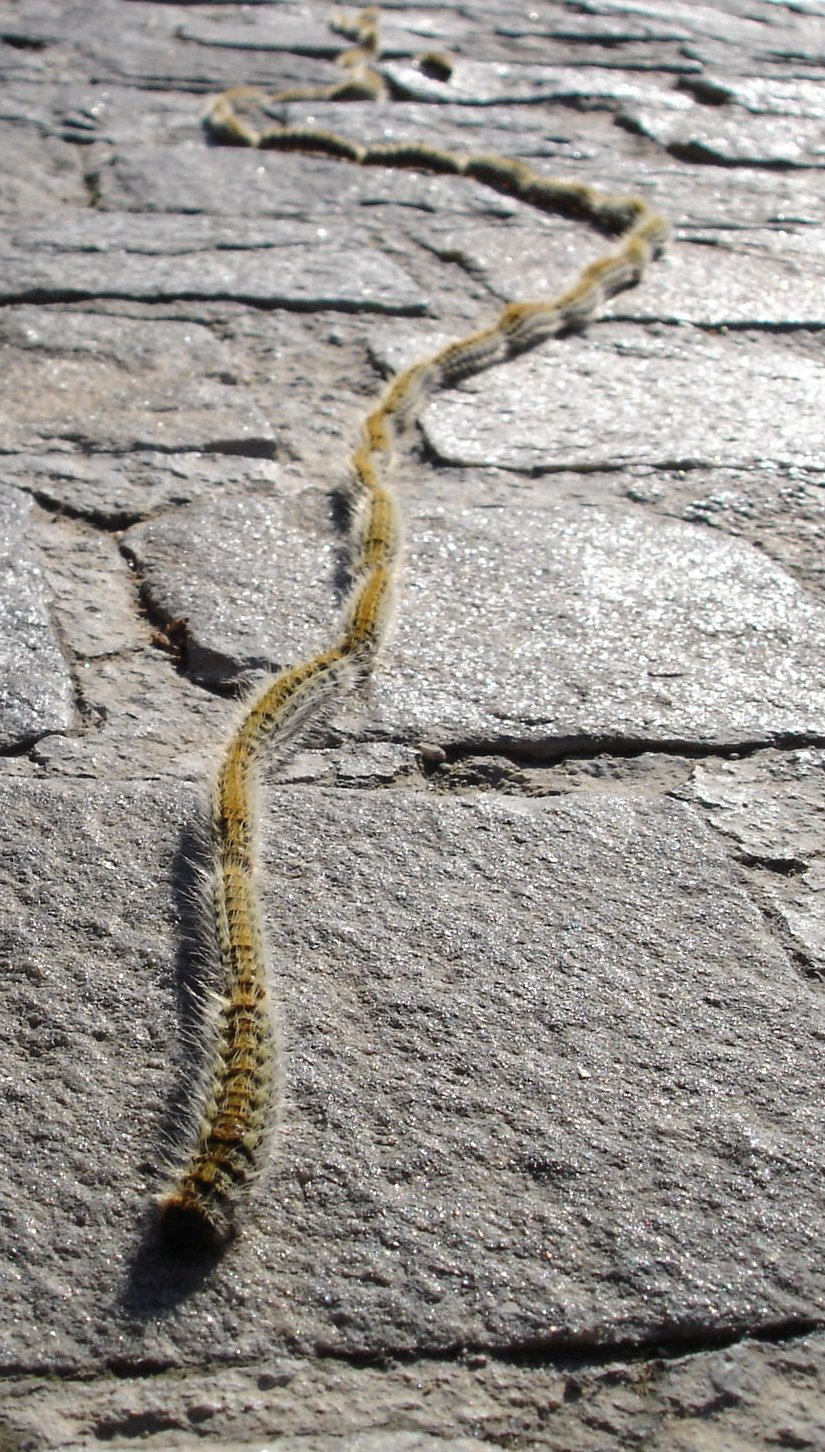
\includegraphics[height=14\baselineskip]{presentation/Thaumetopea_pityocampa_01.jpg}\\
	\vspace{-1.5em}\colorbox{lightgray}{\scriptsize Wikimedia commons}
	\end{flushright}
	\end{columns}
\end{frame}

\end{document}